%%% Template originaly created by Karol Kozioł (mail@karol-koziol.net) and modified for ShareLaTeX use

\documentclass[a4paper,11pt]{article}

\usepackage[T1]{fontenc}
\usepackage[utf8]{inputenc}
\usepackage{graphicx}
\usepackage{xcolor}
\usepackage{tgtermes}
\usepackage{listings}

\usepackage[
pdftitle={CSE258 Homework 2}, 
pdfauthor={Chenyu Huang, University of California San Diego},
colorlinks=true,linkcolor=blue,urlcolor=blue,citecolor=blue,bookmarks=true,
bookmarksopenlevel=2]{hyperref}
\usepackage{amsmath,amssymb,amsthm,textcomp}
\usepackage{enumerate}
\usepackage{multicol}
\usepackage{tikz}

\usepackage{geometry}
\geometry{total={210mm,297mm},
left=25mm,right=25mm,%
bindingoffset=0mm, top=20mm,bottom=20mm}


\linespread{1.3}

\newcommand{\linia}{\rule{\linewidth}{0.5pt}}

% custom theorems if needed
\newtheoremstyle{mytheor}
    {1ex}{1ex}{\normalfont}{0pt}{\scshape}{.}{1ex}
    {{\thmname{#1 }}{\thmnumber{#2}}{\thmnote{ (#3)}}}

\theoremstyle{mytheor}
\newtheorem{defi}{Definition}

% my own titles
\makeatletter
\renewcommand{\maketitle}{
\begin{center}
\vspace{2ex}
{\huge \textsc{\@title}}
\vspace{1ex}
\\
\linia\\
\@author \hfill \@date
\vspace{4ex}
\end{center}
}
\makeatother
%%%

% custom footers and headers
\usepackage{fancyhdr,lastpage}
\pagestyle{fancy}
\lhead{}
\chead{}
\rhead{}
\lfoot{Homework \textnumero{} 2}
\cfoot{}
\rfoot{Page \thepage\ /\ \pageref*{LastPage}}
\renewcommand{\headrulewidth}{0pt}
\renewcommand{\footrulewidth}{0pt}
%

% custom style for code
\lstdefinestyle{customc}{
  belowcaptionskip=1\baselineskip,
  breaklines=true,
  frame=L,
  xleftmargin=\parindent,
  language=C,
  showstringspaces=false,
  basicstyle=\footnotesize\ttfamily,
  keywordstyle=\bfseries\color{green!40!black},
  commentstyle=\itshape\color{purple!40!black},
  identifierstyle=\color{blue},
  stringstyle=\color{orange},
}

\lstdefinestyle{customasm}{
  belowcaptionskip=1\baselineskip,
  frame=L,
  xleftmargin=\parindent,
  language=[x86masm]Assembler,
  basicstyle=\footnotesize\ttfamily,
  commentstyle=\itshape\color{purple!40!black},
}

\lstset{escapechar=@,style=customc}

%%%----------%%%----------%%%----------%%%----------%%%

\begin{document}

\title{CSE258 Homework 2}

\author{Chenyu Huang, University of California San Diego}

\date{02/05/2017}

\maketitle

\section{Classifier evaluation}

\paragraph{Task 1}

After randomly reshuffle the data, the performance for $\lambda=[0, 0.01, 1.0, 100]$ are as follows:
 
\begin{figure}[h]
\centerline{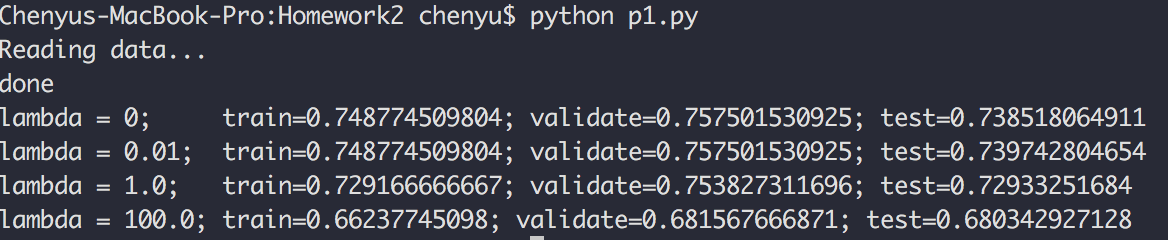
\includegraphics[width=15cm]{p1.png}}
\end{figure}

\paragraph{Task 2}

The number of true positive, true negative, false positive, false negatives and the balanced error rate are as follows:

\begin{figure}[h]
\centerline{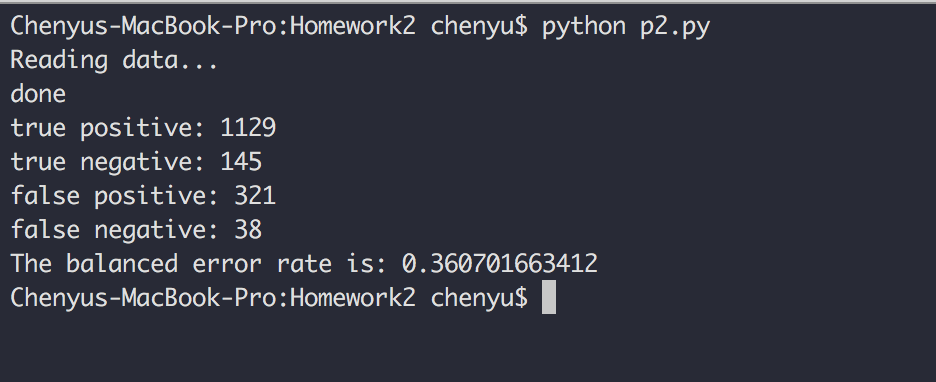
\includegraphics[width=15cm]{p2.png}}
\end{figure}


\paragraph{Task 3}

After sorting the prediction according to confidence, the precision and recall values for $k = [10, 500, 1000]$ predictions are:

\begin{figure}[h]
\centerline{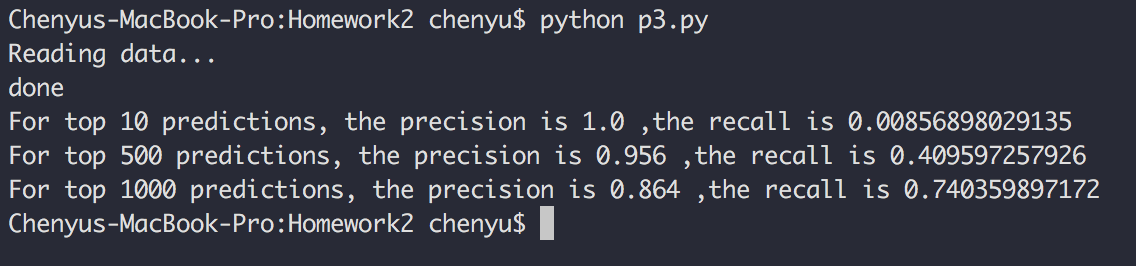
\includegraphics[width=15cm]{p3.png}}
\end{figure}

\paragraph{Task 4}

The precision against recall plot for $k \in [1, len(y\_test)]$ is shown as below:
\begin{figure}[h]
\centerline{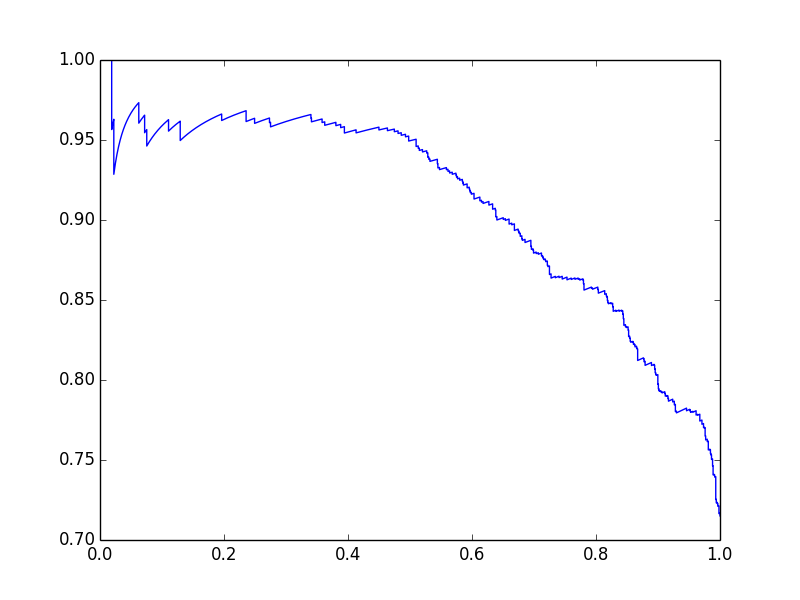
\includegraphics[width=15cm]{p4.png}}
\end{figure}
\clearpage

\section{Dimensionality reduction}

\paragraph{Task 5}
The reconstruction error by replacing each point with their mean vector is: 3675818.61688. This is equivalent to having no principle component


\paragraph{Task 6}
The transform matrix of all 11 principle components are:
\begin{figure}[h]
\centerline{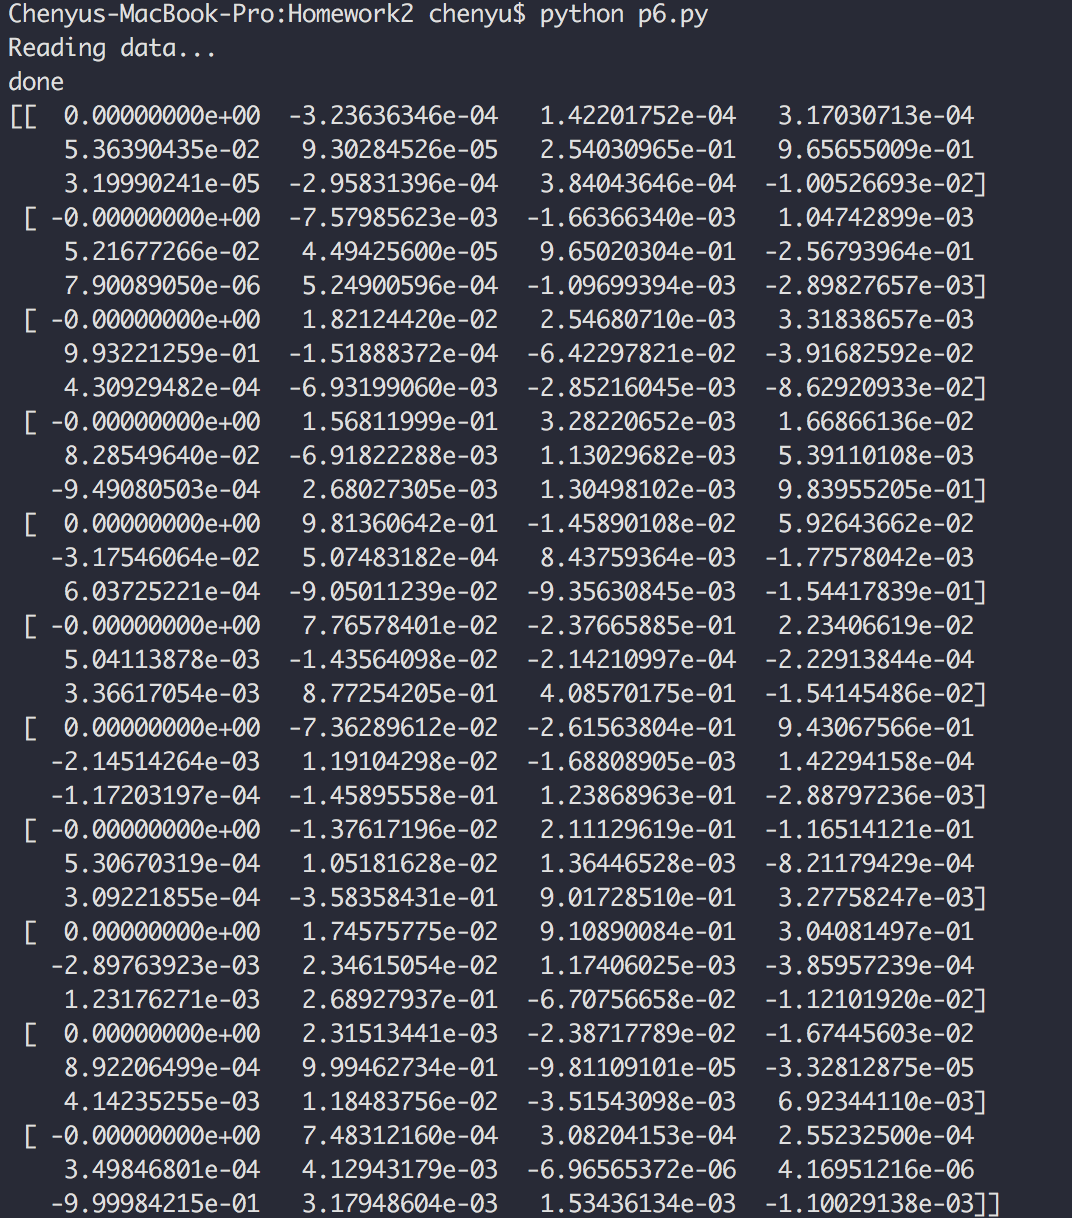
\includegraphics[width=15cm]{p6.png}}
\end{figure}

\paragraph{Task 7}
Using just 4 PCA dimensions, the reconstruction error is: 1345.4755741

\paragraph{Task 8}
The changes on MSE for train and test sets against the number of dimensions used is shown below:

\begin{figure}[h]
\centerline{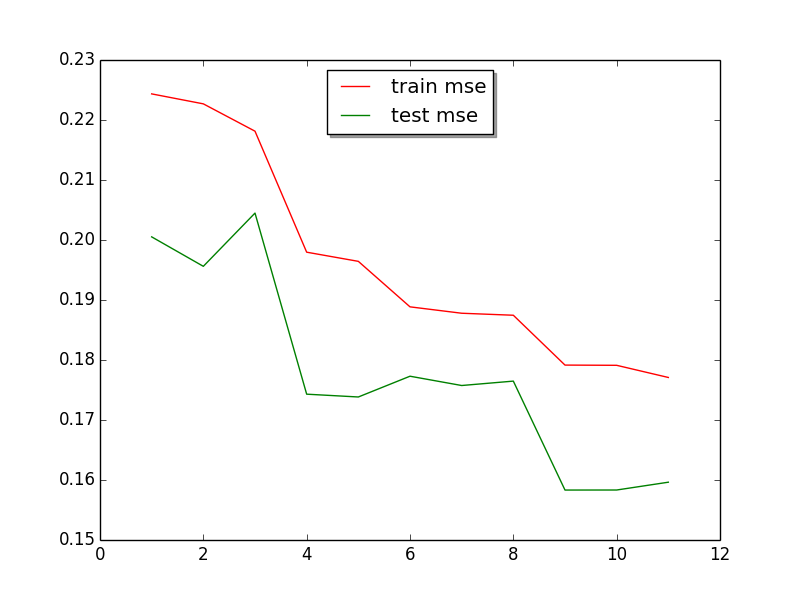
\includegraphics[width=15cm]{p8.png}}
\end{figure}


\clearpage



\clearpage

\section{Code}
\lstinputlisting[language=Python, caption={task1}]{p1.py}\clearpage
\lstinputlisting[language=Python, caption={task2}]{p2.py}\clearpage
\lstinputlisting[language=Python, caption={task3}]{p3.py}\clearpage
\lstinputlisting[language=Python, caption={task4}]{p4.py}\clearpage
\lstinputlisting[language=Python, caption={task5}]{p5.py}\clearpage
\lstinputlisting[language=Python, caption={task6}]{p6.py}\clearpage
\lstinputlisting[language=Python, caption={task7}]{p7.py}\clearpage
\lstinputlisting[language=Python, caption={task8}]{p8.py}\clearpage


\end{document}
